This section presents the experimental results and provides an analysis to assess the performance of both models on the ICH sequence classification.

As discussed in the methodology, each model underwent 10 replicates, comprising a training phase and a testing phase, resulting in a total of 20 observations. It is important to note that the precision values from runs 2 and 7 of the ConvNeXt model were corrupted due to issues with the logging system and will therefore be considered 0 for the analysis.

Additionally, it is worth mentioning that multiclass precision and recall were used, as these metrics provide a more comprehensive view of both model's performance, evaluating their ability to classify both positive and negative cases.

First, the results of each model and metric were analyzed via a Shapiro-Wilk test for normality. Table \ref{tab:shapiro_results} shows the results of the test. For ViVit, all metrics showed a possible normal distribution for an $\alpha = 0.05$. Nevertheless for ConvNeXt, precision wasn't normally distributed.

\begin{table}[h]
    \centering
    \caption{Shapiro-Wilk test results.}
    \renewcommand{\arraystretch}{1.5}
    \begin{tabular}{|c|c|c|c|}
        \hline
        \textbf{Model} & \textbf{Metric} & \textbf{Result} & \textbf{P-value} \\ \hline
        \multirow{3}{*}{ViVit} & Accuracy & Passed & 0.20 \\ \cline{2-4}
                              & Recall & Passed & 0.91 \\ \cline{2-4}
                              & Precision & Passed & 0.91 \\ \hline
        \multirow{3}{*}{ConvNeXt} & Accuracy & Passed & 0.05 \\ \cline{2-4}
                                  & Recall & Passed & 0.16 \\ \cline{2-4}
                                  & Precision & \textcolor{red}{Failed} & 0.01 \\ \hline
    \end{tabular}
    \begin{center}
        \parbox{\columnwidth}{\centering \footnotesize \textbf{Note:} Values are rounded to two decimal places.}
    \end{center}
\label{tab:shapiro_results}
\end{table}

% Values without rounding in case they are needed
% \multirow{3}{*}{ViVit} & Accuracy & Passed & 0.2045 \\ \cline{2-4}
%                       & Recall & Passed & 0.9055 \\ \cline{2-4}
%                       & Precision & Passed & 0.9133 \\ \hline
% \multirow{3}{*}{ConvNeXt} & Accuracy & Passed & 0.0549 \\ \cline{2-4}
%                           & Recall & Passed & 0.1621 \\ \cline{2-4}
%                           & Precision & \textcolor{red}{Failed} & 0.0084 \\ \hline

In terms of the equality of variances, a similar situation to Shapiro-Wilk test happened. This can be observed in table \ref{tab:levene_results}, which shows the Levene's test results. All metrics exhibited a possible equality except for the precision, that had a p-value lower than $\alpha = 0.05$.

\begin{table}[h]
    \centering
    \caption{Levene's test results.}
    \renewcommand{\arraystretch}{1.5}
    \begin{tabular}{|c|c|c|}
        \hline
        \textbf{Metric} & \textbf{Result} & \textbf{P-value} \\ \hline
        Accuracy & Passed & 0.69 \\ \hline
        Recall & Passed & 0.25 \\ \hline
        Precision & \textcolor{red}{Failed} & 0.02 \\ \hline
    \end{tabular}
    \begin{center}
        \parbox{\columnwidth}{\centering \footnotesize \textbf{Note:} Values are rounded to two decimal places.}
    \end{center}
\label{tab:levene_results}
\end{table}

% Values without rounding in case they are needed
% Accuracy & Passed & 0.6906 \\ \hline
% Recall & Passed & 0.2486 \\ \hline
% Precision & \textcolor{red}{Failed} & 0.0170 \\ \hline

A t-test was conducted to assess the significant differences in the metrics of the models, as shown in table \ref{tab:t_results}. Also, the power for each metric is presented using a Cohen's d effect size. For both accuracy and recall, a Student's t-test was used, revealing a significant difference in the results. However, for precision, a Welch's t-test was performed due to unequal variances, despite the fact that the samples for ConvNeXt were not normally distributed. The results indicated no significant difference in precision.

\begin{table}[h]
    \centering
    \caption{T-test results.}
    \renewcommand{\arraystretch}{1.5}
    \begin{tabular}{|c|c|c|c|c|}
        \hline
        \textbf{Metric} & \textbf{Result} & \textbf{P-value} & \textbf{T-value} & \textbf{Power} \\ \hline
        Accuracy & \textcolor{red}{Failed} & 0.00 & 4.20 & 1.00 \\ \hline
        Recall & \textcolor{red}{Failed} & 0.00 & 7.82 & 1.00 \\ \hline
        Precision & Passed & 0.68 & 0.43 & 0.54 \\ \hline
    \end{tabular}
    \begin{center}
        \parbox{\columnwidth}{\centering \footnotesize \textbf{Note:} Values are rounded to two decimal places.}
    \end{center}
\label{tab:t_results}
\end{table}

% Values without rounding in case they are needed
% Accuracy & \textcolor{red}{Failed} & 0.0005 & 4.2054 & 0.9998 \\ \hline
% Recall & \textcolor{red}{Failed} & 0.0000 & 7.8191 & 1.0000 \\ \hline
% Precision & Passed & 0.6784 & 0.4256 & 0.5369 \\ \hline

Since the precision samples for ConvNeXt were not normally distributed and the power of the t-test was reduced, we opted to perform a non-parametric test for all metrics to strengthen the validity of the subsequent analysis. The Mann-Whitney U test was conducted, and its results were consistent with those of the parametric t-test. These findings are presented in table \ref{tab:mann_whitney_results}.

\begin{table}[h]
    \centering
    \caption{Mann-Whitney U test results.}
    \renewcommand{\arraystretch}{1.5}
    \begin{tabular}{|c|c|c|c|c|}
        \hline
        \textbf{Metric} & \textbf{Result} & \textbf{P-value} & \textbf{U-value} \\ \hline
        Accuracy & \textcolor{red}{Failed} & 0.00 & 95.00 \\ \hline
        Recall & \textcolor{red}{Failed} & 0.00 & 99.50 \\ \hline
        Precision & Passed & 1.00 & 50.00 \\ \hline
    \end{tabular}
    \begin{center}
        \parbox{\columnwidth}{\centering \footnotesize \textbf{Note:} Values are rounded to two decimal places.}
    \end{center}
\label{tab:mann_whitney_results}
\end{table}

% Values without rounding in case they are needed
% Accuracy & \textcolor{red}{Failed} & 0.0006 & 95.0000 \\ \hline
% Recall & \textcolor{red}{Failed} & 0.0002 & 99.5000 \\ \hline
% Precision & Passed & 1.0000 & 50.0000 \\ \hline

Figure \ref{fig:accuracy_bloxplot} shows a boxplot representing each model's performance on the accuracy. It is evident that ViVit outperformed ConvNeXt on this metric, exhibiting higher minimum, maximum, and median values. While both models exhibit similar variance, most of ViVit's observations are above 0.65, whereas the majority of ConvNeXT's observations fall below this threshold. This suggests that ViVit may have had a greater ability to accurately classify ICH sequences.

\begin{figure}[h]
    \centering
    \scalebox{0.7}{% This file was created with tikzplotlib v0.10.1.
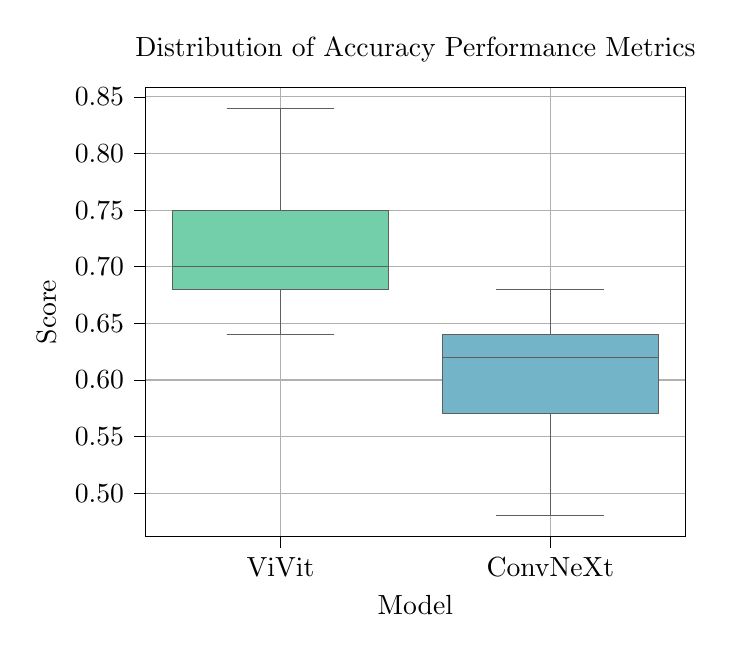
\begin{tikzpicture}

\definecolor{darkgray176}{RGB}{176,176,176}
\definecolor{dimgray95}{RGB}{95,95,95}
\definecolor{mediumaquamarine115206170}{RGB}{115,206,170}
\definecolor{mediumaquamarine116180200}{RGB}{116,180,200}

\begin{axis}[
tick align=outside,
tick pos=left,
title={Distribution of Accuracy Performance Metrics},
x grid style={darkgray176},
xlabel={Model},
xmajorgrids,
xmin=-0.5, xmax=1.5,
xtick style={color=black},
xtick={0,1},
xticklabels={ViVit,ConvNeXt},
y grid style={darkgray176},
ylabel={Score},
ymajorgrids,
ymin=0.462, ymax=0.858,
ytick style={color=black},
ytick={0.45,0.5,0.55,0.6,0.65,0.7,0.75,0.8,0.85,0.9},
yticklabels={
  \(\displaystyle {0.45}\),
  \(\displaystyle {0.50}\),
  \(\displaystyle {0.55}\),
  \(\displaystyle {0.60}\),
  \(\displaystyle {0.65}\),
  \(\displaystyle {0.70}\),
  \(\displaystyle {0.75}\),
  \(\displaystyle {0.80}\),
  \(\displaystyle {0.85}\),
  \(\displaystyle {0.90}\)
}
]
\path [draw=dimgray95, fill=mediumaquamarine115206170]
(axis cs:-0.4,0.68)
--(axis cs:0.4,0.68)
--(axis cs:0.4,0.75)
--(axis cs:-0.4,0.75)
--(axis cs:-0.4,0.68)
--cycle;
\addplot [dimgray95]
table {%
0 0.68
0 0.64
};
\addplot [dimgray95]
table {%
0 0.75
0 0.84
};
\addplot [dimgray95]
table {%
-0.2 0.64
0.2 0.64
};
\addplot [dimgray95]
table {%
-0.2 0.84
0.2 0.84
};
\path [draw=dimgray95, fill=mediumaquamarine116180200]
(axis cs:0.6,0.57)
--(axis cs:1.4,0.57)
--(axis cs:1.4,0.64)
--(axis cs:0.6,0.64)
--(axis cs:0.6,0.57)
--cycle;
\addplot [dimgray95]
table {%
1 0.57
1 0.48
};
\addplot [dimgray95]
table {%
1 0.64
1 0.68
};
\addplot [dimgray95]
table {%
0.8 0.48
1.2 0.48
};
\addplot [dimgray95]
table {%
0.8 0.68
1.2 0.68
};
\addplot [dimgray95]
table {%
-0.4 0.7
0.4 0.7
};
\addplot [dimgray95]
table {%
0.6 0.62
1.4 0.62
};
\end{axis}

\end{tikzpicture}
}
    \caption{Accuracy boxplots.}
    \label{fig:accuracy_bloxplot}
\end{figure}

Similarly, Figure \ref{fig:precision_bloxplot} presents the boxplot representation of each model’s performance on precision. However, the results here are more complex. Both models achieved a maximum of score of 1, but ViVit’s minimum score is significantly higher than ConvNeXt's, resulting in a much higher variance for the latter. While the median scores for both models were relatively close, ConvNeXt’s median is notably higher.

\begin{figure}[h]
    \centering
    \scalebox{0.7}{% This file was created with tikzplotlib v0.10.1.
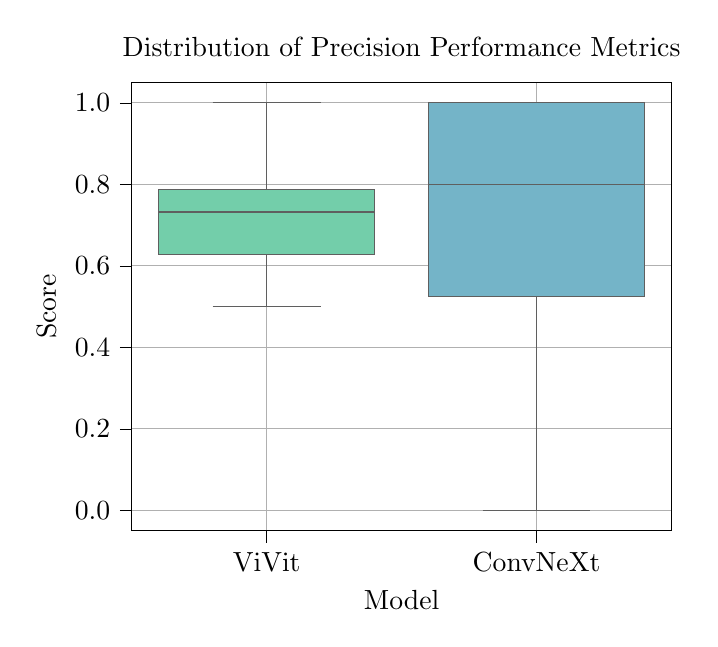
\begin{tikzpicture}

\definecolor{darkgray176}{RGB}{176,176,176}
\definecolor{dimgray95}{RGB}{95,95,95}
\definecolor{mediumaquamarine115206170}{RGB}{115,206,170}
\definecolor{mediumaquamarine116180200}{RGB}{116,180,200}

\begin{axis}[
tick align=outside,
tick pos=left,
title={Distribution of Precision Performance Metrics},
x grid style={darkgray176},
xlabel={Model},
xmajorgrids,
xmin=-0.5, xmax=1.5,
xtick style={color=black},
xtick={0,1},
xticklabels={ViVit,ConvNeXt},
y grid style={darkgray176},
ylabel={Score},
ymajorgrids,
ymin=-0.05, ymax=1.05,
ytick style={color=black},
ytick={-0.2,0,0.2,0.4,0.6,0.8,1,1.2},
yticklabels={
  \(\displaystyle {\ensuremath{-}0.2}\),
  \(\displaystyle {0.0}\),
  \(\displaystyle {0.2}\),
  \(\displaystyle {0.4}\),
  \(\displaystyle {0.6}\),
  \(\displaystyle {0.8}\),
  \(\displaystyle {1.0}\),
  \(\displaystyle {1.2}\)
}
]
\path [draw=dimgray95, fill=mediumaquamarine115206170]
(axis cs:-0.4,0.627840909090909)
--(axis cs:0.4,0.627840909090909)
--(axis cs:0.4,0.7875)
--(axis cs:-0.4,0.7875)
--(axis cs:-0.4,0.627840909090909)
--cycle;
\addplot [dimgray95]
table {%
0 0.627840909090909
0 0.5
};
\addplot [dimgray95]
table {%
0 0.7875
0 1
};
\addplot [dimgray95]
table {%
-0.2 0.5
0.2 0.5
};
\addplot [dimgray95]
table {%
-0.2 1
0.2 1
};
\path [draw=dimgray95, fill=mediumaquamarine116180200]
(axis cs:0.6,0.525)
--(axis cs:1.4,0.525)
--(axis cs:1.4,1)
--(axis cs:0.6,1)
--(axis cs:0.6,0.525)
--cycle;
\addplot [dimgray95]
table {%
1 0.525
1 0
};
\addplot [dimgray95]
table {%
1 1
1 1
};
\addplot [dimgray95]
table {%
0.8 0
1.2 0
};
\addplot [dimgray95]
table {%
0.8 1
1.2 1
};
\addplot [dimgray95]
table {%
-0.4 0.732142857142857
0.4 0.732142857142857
};
\addplot [dimgray95]
table {%
0.6 0.8
1.4 0.8
};
\end{axis}

\end{tikzpicture}
}
    \caption{Precision boxplots.}
    \label{fig:precision_bloxplot}
\end{figure}

This results suggests that although ConvNeXt may have had a greater potential for correct predictions, it also showed more variability and inconsistency in its results.

\begin{figure}[h]
    \centering
    \scalebox{0.7}{% This file was created with tikzplotlib v0.10.1.
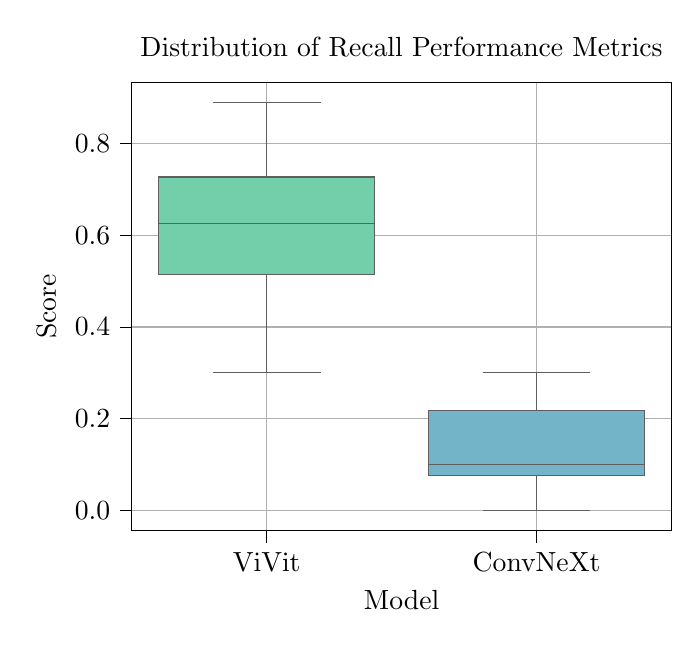
\begin{tikzpicture}

\definecolor{darkgray176}{RGB}{176,176,176}
\definecolor{dimgray95}{RGB}{95,95,95}
\definecolor{mediumaquamarine115206170}{RGB}{115,206,170}
\definecolor{mediumaquamarine116180200}{RGB}{116,180,200}

\begin{axis}[
tick align=outside,
tick pos=left,
title={Distribution of Recall Performance Metrics},
x grid style={darkgray176},
xlabel={Model},
xmajorgrids,
xmin=-0.5, xmax=1.5,
xtick style={color=black},
xtick={0,1},
xticklabels={ViVit,ConvNeXt},
y grid style={darkgray176},
ylabel={Score},
ymajorgrids,
ymin=-0.0444444444444444, ymax=0.933333333333333,
ytick style={color=black},
ytick={-0.2,0,0.2,0.4,0.6,0.8,1},
yticklabels={
  \(\displaystyle {\ensuremath{-}0.2}\),
  \(\displaystyle {0.0}\),
  \(\displaystyle {0.2}\),
  \(\displaystyle {0.4}\),
  \(\displaystyle {0.6}\),
  \(\displaystyle {0.8}\),
  \(\displaystyle {1.0}\)
}
]
\path [draw=dimgray95, fill=mediumaquamarine115206170]
(axis cs:-0.4,0.513888888888889)
--(axis cs:0.4,0.513888888888889)
--(axis cs:0.4,0.727272727272727)
--(axis cs:-0.4,0.727272727272727)
--(axis cs:-0.4,0.513888888888889)
--cycle;
\addplot [dimgray95]
table {%
0 0.513888888888889
0 0.3
};
\addplot [dimgray95]
table {%
0 0.727272727272727
0 0.888888888888889
};
\addplot [dimgray95]
table {%
-0.2 0.3
0.2 0.3
};
\addplot [dimgray95]
table {%
-0.2 0.888888888888889
0.2 0.888888888888889
};
\path [draw=dimgray95, fill=mediumaquamarine116180200]
(axis cs:0.6,0.0762987012987013)
--(axis cs:1.4,0.0762987012987013)
--(axis cs:1.4,0.21875)
--(axis cs:0.6,0.21875)
--(axis cs:0.6,0.0762987012987013)
--cycle;
\addplot [dimgray95]
table {%
1 0.0762987012987013
1 0
};
\addplot [dimgray95]
table {%
1 0.21875
1 0.3
};
\addplot [dimgray95]
table {%
0.8 0
1.2 0
};
\addplot [dimgray95]
table {%
0.8 0.3
1.2 0.3
};
\addplot [dimgray95]
table {%
-0.4 0.625874125874126
0.4 0.625874125874126
};
\addplot [dimgray95]
table {%
0.6 0.1
1.4 0.1
};
\end{axis}

\end{tikzpicture}
}
    \caption{Recall boxplots.}
    \label{fig:recall_bloxplot}
\end{figure}

Once again, Figure \ref{fig:recall_bloxplot} shows a boxplot representation of each model’s performance, this time on the recall metric. The results are similar to those in Figure \ref{fig:accuracy_bloxplot}, with ViVit showing higher minimum, maximum, and median values than ConvNeXT. Although ConvNeXT exhibits lower variance, all its observations fall below 0.4, while most of ViVit's observations exceed this threshold. This indicates poorer performance by ConvNeXT, as the consistently low recall values may indicate a higher tendency for the model to misclassify sequences.

Table \ref{tab:min_max_metrics} provides a summary of the results shown in the boxplots, detailing the specific minimum and maximum values achieved by each model. Notably, Meanwhile, Table \ref{tab:mean_metrics} highlights the mean values, emphasizing ViVit's superiority across all three metrics. However, it is important to note that the mean scores were significantly influenced by outliers.

\begin{table}[h]
    \centering
    \caption{Min and max metrics of each model.}
    \renewcommand{\arraystretch}{1.5}
    \begin{tabular}{|c|c|c|c|c|c|c|}
        \hline
        \multirow{2}{*}{\textbf{Model}} & \multicolumn{2}{|c|}{\textbf{Accuracy}} & \multicolumn{2}{|c|}{\textbf{Precision}} & \multicolumn{2}{|c|}{\textbf{Recall}} \\ \cline{2-7}
                               & Min  & Max   & Min  & Max   & Min  & Max   \\ \hline
        ViVit                  & \textbf{0.64} & \textbf{0.84}  & \textbf{0.50} & \textbf{1.00}  & \textbf{0.30} & \textbf{0.89}  \\ \hline
        ConvNeXt               & 0.48 & 0.68  & 0.00 & \textbf{1.00} & 0.00 & 0.30  \\ \hline
    \end{tabular}
    \begin{center}
        \parbox{\columnwidth}{\centering \footnotesize \textbf{Note:} Values are rounded to two decimal places.}
    \end{center}
    \label{tab:min_max_metrics}
\end{table}


\begin{table}[h]
    \centering
    \caption{Mean metrics of each model.}
    \renewcommand{\arraystretch}{1.5}
    \begin{tabular}{|c|c|c|c|}
        \hline
        \textbf{Model}     & \textbf{Accuracy}     & \textbf{Precision}     & \textbf{Recall}     \\ \hline
        ViVit     & \textbf{0.72}         & \textbf{0.73}          & \textbf{0.62}       \\ \hline
        ConvNeXt  & 0.60         & 0.67          & 0.13       \\ \hline
    \end{tabular}
    \begin{center}
        \parbox{\columnwidth}{\centering \footnotesize \textbf{Note:} Values are rounded to two decimal places.}
    \end{center}
    \label{tab:mean_metrics}
\end{table}

\begin{figure}[h]
    \centering
    \scalebox{0.7}{% This file was created with tikzplotlib v0.10.1.
\begin{tikzpicture}

\definecolor{darkgray176}{RGB}{176,176,176}
\definecolor{darkslategray38}{RGB}{38,38,38}

\begin{axis}[
tick align=outside,
tick pos=left,
title={Mean Confusion Matrix for ViViT},
x grid style={darkgray176},
xlabel={Predicted Label},
xmin=0, xmax=2,
xtick style={color=black},
xtick={0.5,1.5},
xticklabels={Negative,Positive},
y dir=reverse,
y grid style={darkgray176},
ylabel={True Label},
ymin=0, ymax=2,
ytick style={color=black},
ytick={0.5,1.5},
yticklabel style={rotate=90.0},
yticklabels={Negative,Positive}
]
\addplot graphics [includegraphics cmd=\pgfimage,xmin=0, xmax=2, ymin=2, ymax=0] {imgs/tikz/mean_confusion_matrix_for_vivit-000.png};
\draw (axis cs:0.5,0.5) node[
  scale=0.9,
  text=white,
  rotate=0.0
]{11.20};
\draw (axis cs:1.5,0.5) node[
  scale=0.9,
  text=darkslategray38,
  rotate=0.0
]{3.00};
\draw (axis cs:0.5,1.5) node[
  scale=0.9,
  text=darkslategray38,
  rotate=0.0
]{4.10};
\draw (axis cs:1.5,1.5) node[
  scale=0.9,
  text=darkslategray38,
  rotate=0.0
]{6.70};
\end{axis}

\end{tikzpicture}
}
    \caption{Mean confusion matrix of ViVit.}
    \label{fig:mean_cm_vivit}
\end{figure}

\begin{figure}[h]
    \centering
    \scalebox{0.7}{\input{imgs/tikz/mean_confusion_matrix_for_ConvNeXt}}
    \caption{Mean confusion matrix of ConvNeXt.}
    \label{fig:mean_cm_ConvNeXt}
\end{figure}

On the other hand, Figures \ref{fig:mean_cm_vivit} and \ref{fig:mean_cm_ConvNeXt} display the confusion matrices for ViVit and ConvNeXt, respectively. A key focus here is the number of false negatives, as these can lead to missed diagnoses, potentially overlooking the presence of ICH and resulting in fatal consequences for patients. ViVit significantly outperformed ConvNeXt in this regard, producing less than half the number of false negatives.

Additionally, ViVit correctly predicted positive cases more than four times as often as ConvNeXt. However, it is also notable that ConvNeXt correctly predicted more negative cases than ViVit and produced six times fewer false positives.

Having correctly analyzed the results obtained, we now proceed to draw our conclusions and offer recommendations for future studies on ICH sequence classification.